\documentclass[11pt]{article}
\usepackage[T1]{fontenc}
\usepackage[utf8]{inputenc}
\usepackage[margin=1in]{geometry}
\usepackage{amsmath,amssymb,amsthm,microtype}
\usepackage{tikz}
\usepackage{float}
\usepackage[hidelinks]{hyperref}
\newtheorem{proposition}{Proposition}
\newtheorem{lemma}{Lemma}
\newtheorem{corollary}{Corollary}
\title{Threshold policies for the fluid forgetting model}
\author{Analytical research note}
\date{27 September 2026}
\begin{document}
\maketitle

This note proves the threshold structure for the fluid model with the exact
Beta demand. The argument uses no numerical approximation. It concerns the
continuous-time control problem; a corresponding theorem for the original
stochastic Bellman equation does not follow from this proof.

\section*{Derivation of the fluid model}
Assume
\begin{equation*}
0<p_1<p_2<1,\quad 0\le c_1<c_2<R,\quad
0<p_0<1,\quad 0<\rho,\gamma<1.
\end{equation*}
As in the fluid progress note, we use the normalized coordinate
$x=(1-\rho)S\in[0,1]$ and write
\begin{equation*}
\lambda=-\log\rho,\qquad \delta=-\log\gamma,\qquad
\Delta p=p_2-p_1,\qquad \Delta c=c_2-c_1.
\end{equation*}
On the mature boundary, the probability of a purchase is
\begin{equation*}
D(x)=1-I_{p_0}\!\left(1+\frac{x}{1-\rho},
                         1+\frac{1-x}{1-\rho}\right).
\end{equation*}
Here $I_z(a,b)$ is the regularized incomplete beta function. Under
product $i$, a purchase yields profit $R-c_i$ and succeeds with probability
$p_i$. If no purchase occurs, the state stays at $x$.

\subsection*{Fluid Bellman for $V$}
Write $V$ for the value when the product is chosen optimally.
Following the fluid progress note, consider the transitions over a
small time step $dt$:
\begin{equation*}
T^s_{dt}(x)=\rho^{dt}x+(1-\rho^{dt}),\qquad
T^f_{dt}(x)=\rho^{dt}x.
\end{equation*}
Over this step, the profit per purchase under product $i$ is $(R-c_i)dt$
and the discount factor is $\gamma^{dt}$. We keep $D(x)$ fixed at the
original $\rho$ as $dt\to0$.
Since
\begin{align*}
\rho^{dt}&=e^{-\lambda dt}=1-\lambda dt+o(dt),\\
\gamma^{dt}&=e^{-\delta dt}=1-\delta dt+o(dt),
\end{align*}
the state increments are
\begin{align*}
T^s_{dt}(x)-x&=\lambda(1-x)dt+o(dt),\\
T^f_{dt}(x)-x&=-\lambda xdt+o(dt).
\end{align*}
Under product $i$, the expected change in the state is
\begin{equation*}
D(x)\bigl[p_i\lambda(1-x)+(1-p_i)(-\lambda x)\bigr]dt+o(dt)
=D(x)\lambda(p_i-x)dt+o(dt).
\end{equation*}
Thus the fluid state equation and profit rate are
\begin{equation}\label{eq:fluid-dynamics}
\dot x=D(x)\lambda(p_i-x),\qquad D(x)(R-c_i).
\end{equation}

To keep the notation simple, we use $V$ at both the discrete and fluid
stages of the following formal first-order derivation. The Bellman
equation over $dt$ is
\begin{equation}\label{eq:scaled-bellman}
\begin{aligned}
V(x)={}&(1-D(x))\gamma^{dt}V(x)\\
&+D(x)\max_{i\in\{1,2\}}\left\{(R-c_i)dt+\gamma^{dt}
\left[p_iV(T^s_{dt}(x))+(1-p_i)V(T^f_{dt}(x))\right]\right\}.
\end{aligned}
\end{equation}
Taylor expansion gives
\begin{align*}
V(T^s_{dt}(x))&=V(x)+\lambda(1-x)V'(x)dt+o(dt),\\
V(T^f_{dt}(x))&=V(x)-\lambda xV'(x)dt+o(dt).
\end{align*}
Combining the success and failure terms,
\begin{equation*}
p_iV(T^s_{dt}(x))+(1-p_i)V(T^f_{dt}(x))
=V(x)+\lambda(p_i-x)V'(x)dt+o(dt).
\end{equation*}
Substituting this and $\gamma^{dt}=1-\delta dt+o(dt)$ into
\eqref{eq:scaled-bellman} and collecting terms,
\begin{align*}
V(x)=V(x)+\Bigl[
D(x)\max_{i\in\{1,2\}}\{R-c_i+\lambda(p_i-x)V'(x)\}
-\delta V(x)\Bigr]dt+o(dt).
\end{align*}

Cancelling $V(x)$, dividing by $dt$, and letting $dt\to0$ yields
\begin{equation}\label{eq:fluid-HJB}
\delta V(x)=D(x)\max_{i\in\{1,2\}}
\{R-c_i+\lambda(p_i-x)V'(x)\}.
\end{equation}
To obtain the discounted profit representation, let $i(t)$ denote any
admissible product choice and let $x(t)$ follow
\eqref{eq:fluid-dynamics}, starting at $x(0)=x$. Since
\eqref{eq:fluid-HJB} takes the maximum over products, wherever $V$ is
differentiable we have
\begin{equation*}
\delta V(x(t))
\ge D(x(t))(R-c_{i(t)})+V'(x(t))\dot x(t).
\end{equation*}
Multiplying by $e^{-\delta t}$ and using the chain rule gives
\begin{align*}
\frac{d}{dt}\bigl[e^{-\delta t}V(x(t))\bigr]
&=e^{-\delta t}\bigl[V'(x(t))\dot x(t)-\delta V(x(t))\bigr]\\
&\le -e^{-\delta t}D(x(t))(R-c_{i(t)}).
\end{align*}

Integrating from $0$ to $T$,
\begin{equation*}
e^{-\delta T}V(x(T))-V(x)
\le -\int_0^T e^{-\delta t}D(x(t))(R-c_{i(t)})\,dt.
\end{equation*}
Rearranging,
\begin{equation*}
V(x)\ge
\int_0^T e^{-\delta t}D(x(t))(R-c_{i(t)})\,dt
+e^{-\delta T}V(x(T)).
\end{equation*}
Because $V$ is bounded and $\delta>0$, the terminal term tends to zero
as $T\to\infty$. Thus $V(x)$ is at least the discounted profit of every
admissible policy. For an admissible policy attaining the Bellman maximum
along its trajectory, these inequalities become equalities. This includes
holding mixtures of tied maximizing products, as described below.
The chain-rule calculation applies where $V$ is differentiable; at
corners, dynamic programming supplies the corresponding argument.
Consequently, the fluid value is the largest discounted profit over
these trajectories:
\begin{equation}\label{eq:fluid-value}
V(x)=\sup\int_0^\infty e^{-\delta t}D(x(t))(R-c_{i(t)})\,dt,
\qquad x(0)=x.
\end{equation}
We also allow mixtures:
both the drift and the profit rate are averaged using the same product
fractions. In particular, at $x\in[p_1,p_2]$, the product-2 fraction
\begin{equation*}
\frac{x-p_1}{p_2-p_1}
\end{equation*}
makes the average drift zero and holds the state at $x$. Maximizing over
mixtures gives the same Bellman equation, because both drift and profit
depend linearly on the fractions.

Where $V$ is differentiable, product 2 is strictly preferred when
\begin{align*}
R-c_2+\lambda(p_2-x)V'(x)
&>R-c_1+\lambda(p_1-x)V'(x)\\
\Longleftrightarrow\qquad V'(x)&>\frac{\Delta c}{\lambda\Delta p}.
\end{align*}
The Taylor derivation applies where the derivatives exist; the threshold
proof below does not assume that $V$ is differentiable everywhere.
The proposition establishes the global policy structure for this fluid
problem, including holding mixtures at attractive thresholds.

\begin{proposition}[At most one interval of product 2]\label{prop:fluid-band}
The fluid problem admits an optimal stationary policy with numbers
$0\le x_L\le x_H\le1$ such that, away from threshold states,
\begin{equation*}
i(x)=
\begin{cases}
1,&x<x_L,\\
2,&x_L<x<x_H,\\
1,&x>x_H.
\end{cases}
\end{equation*}
Empty intervals are allowed. Thus the nonconstant action patterns, in
increasing order of the state, are
\begin{equation*}
1\longrightarrow2,\qquad 2\longrightarrow1,\qquad
1\longrightarrow2\longrightarrow1.
\end{equation*}
Constant policies are also possible. There cannot be two separated regions
of strict preference for product 2, such as a strict $2\to1\to2$ pattern.
At an attractive threshold in $(p_1,p_2)$ the optimal prescription includes
the holding mixture. Choices at indifference points are made consistently
with the stated interval policy.
\end{proposition}

The proof has two parts. First, a shape property of the Beta demand limits
the transformed payoff to at most one valley followed by one peak. Second,
the one-dimensional control problem then has at most one interval on which
product 2 is optimal. Neither part assumes that the optimal value is
continuously differentiable everywhere.

\section*{1. An exact transformation}
We want to rewrite the objective so that the product choice enters only
through the movement of the state. To find the right adjustment, compare
the two products at the same state $x$. Choosing product 2 reduces the
current profit rate by $D(x)\Delta c$ and increases the state drift by
$\lambda D(x)\Delta p$. Their ratio is
\begin{equation*}
\frac{D(x)\Delta c}{\lambda D(x)\Delta p}
=\frac{\Delta c}{\lambda\Delta p}.
\end{equation*}
This ratio is independent of $x$. It suggests crediting each extra unit
of state accumulation at the rate $\Delta c/(\lambda\Delta p)$, so that
the extra drift exactly offsets the extra product cost.

To see the cancellation explicitly, the two products satisfy
\begin{equation*}
c_i=c_1+\frac{\Delta c}{\Delta p}(p_i-p_1),
\qquad i\in\{1,2\}.
\end{equation*}
Adding the state credit to the profit rate and using
$\dot x=\lambda D(x)(p_i-x)$ gives
\begin{align*}
D(x)(R-c_i)+\frac{\Delta c}{\lambda\Delta p}\dot x
&=D(x)\left[R-c_i+\frac{\Delta c}{\Delta p}(p_i-x)\right]\\
&=D(x)\left[R-c_1+\frac{\Delta c}{\Delta p}(p_1-x)\right].
\end{align*}
The last expression is the same for either product. Rearranging,
\begin{equation*}
D(x)(R-c_i)
=D(x)\left[R-c_1+\frac{\Delta c}{\Delta p}(p_1-x)\right]
-\frac{\Delta c}{\lambda\Delta p}\dot x.
\end{equation*}
The first term now depends only on the state; the product choice affects
the second term through $\dot x$. The same identity holds for mixtures,
since both the drift and the profit are averaged with the same fractions.

Next, remove the term involving $\dot x$ from the discounted objective.
For a trajectory starting at $x(0)=x$, integration by parts gives
\begin{align*}
\int_0^T e^{-\delta t}\dot x(t)\,dt
&=\bigl[e^{-\delta t}x(t)\bigr]_0^T
+\delta\int_0^T e^{-\delta t}x(t)\,dt\\
&=e^{-\delta T}x(T)-x
+\delta\int_0^T e^{-\delta t}x(t)\,dt.
\end{align*}

Since $x(T)\in[0,1]$ and $\delta>0$, the terminal term vanishes as
$T\to\infty$. Therefore,
\begin{equation*}
-\frac{\Delta c}{\lambda\Delta p}
\int_0^\infty e^{-\delta t}\dot x(t)\,dt
=\frac{\Delta c}{\lambda\Delta p}x
-\frac{\delta\Delta c}{\lambda\Delta p}
\int_0^\infty e^{-\delta t}x(t)\,dt.
\end{equation*}
Combining this with the rewritten profit rate identifies the payoff
that remains inside the integral:
\begin{equation}\label{eq:F}
F(x)=D(x)\left[R-c_1+\frac{\Delta c}{\Delta p}(p_1-x)\right]
       -\frac{\delta\Delta c}{\lambda\Delta p}x.
\end{equation}
Thus the first term in $F$ is the common payoff obtained after crediting
state accumulation. The second is the discount correction generated by
integration by parts. This is how the definition of $F$ is obtained.

For every admissible policy, its discounted profit equals the initial
state credit plus the discounted integral of $F$ along its trajectory.
Taking the supremum over policies yields
\begin{equation}\label{eq:transform}
V(x)=\frac{\Delta c}{\lambda\Delta p}x+
       \sup\int_0^\infty e^{-\delta t}F(x(t))\,dt.
\end{equation}
For a given initial state, the first term is the same for every policy,
so the transformation preserves their ranking.

For the proof, write
$W(x)=V(x)-\Delta c\,x/(\lambda\Delta p)$.
Then $W$ is the value of maximizing the discounted integral of $F$.
Where the derivative exists,
\begin{equation*}
V'(x)=W'(x)+\frac{\Delta c}{\lambda\Delta p}.
\end{equation*}
Substituting into \eqref{eq:fluid-HJB} and using the same cancellation
gives its control equation:
\begin{equation}\label{eq:W-HJB}
\delta W(x)=F(x)+\max_{i=1,2}
             \{\lambda D(x)(p_i-x)W'(x)\}.
\end{equation}
Where the derivative exists, product 2 is strictly optimal precisely
when $W'>0$, and product 1 is strictly optimal when $W'<0$.
The transformed flow payoff is the same for both products at a given
state. Products determine the direction and speed of movement through
the graph of $F$, which is why studying the shape of this single function
helps us characterize the optimal policy.

\section*{2. The Beta demand has the required shape}
\begin{lemma}[Shape of the exact Beta demand]\label{lem:beta-marginal-demand}
Let $0<p_0<1$, $0<\rho<1$, and $n=(1-\rho)^{-1}$. For
\begin{equation*}
D(x)=1-I_{p_0}\bigl(1+nx,1+n(1-x)\bigr),\qquad 0\le x\le1,
\end{equation*}
we have $D'(x)>0$ and
\begin{equation*}
D'(x)D'''(x)-[D''(x)]^2<0.
\end{equation*}
In particular, $D'$ is strictly log-concave. The endpoint derivatives are
understood through the smooth extension of $D$.
\end{lemma}

\begin{proof}
We establish a fixed-total Beta identity first. In this proof only, fix
$N>2$ and $p\in(0,1)$, write $b=N-a$, and let
\begin{equation*}
S(a)=1-I_p(a,b),\qquad 0<a<N.
\end{equation*}
For $0<h<b$, take a Dirichlet random vector $(U,Y,W)$ with parameters
$(a,h,b-h)$. Then $U$ has the Beta$(a,b)$ distribution, whereas $U+Y$
has the Beta$(a+h,b-h)$ distribution. Since $U+Y=1-W\ge U$,
\begin{equation*}
S(a+h)-S(a)=\Pr(U<p,\ W<1-p).
\end{equation*}
Integrating the Dirichlet density over this rectangle, dividing by $h$,
and letting $h\downarrow0$ gives
\begin{equation}\label{eq:beta-flux-positive}
S'(a)=\frac1{B(a,b)}
\int_0^p\int_0^{1-p}
\frac{u^{a-1}w^{b-1}}{1-u-w}\,dw\,du>0.
\end{equation}
Here $h\Gamma(h)\to1$. Dominated convergence is valid: the corner
singularity is proportional to
$\bigl[(p-u)+(1-p-w)\bigr]^{-1}$, which is integrable in two dimensions.
Choosing a fixed $h_0<b$ bounds the remaining integrand by a constant
times $u^{a-1}w^{b-h_0-1}/(1-u-w)$, also integrable.

Expand $(1-u-w)^{-1}$ into its nonnegative geometric series and use the
binomial theorem. Tonelli's theorem applied to
\eqref{eq:beta-flux-positive} yields
\begin{equation}\label{eq:beta-flux-series}
S'(a)=\sum_{j,k\ge0}t_{jk}(a),\qquad
 t_{jk}(a)=
\frac{p^a(1-p)^b}{B(a,b)}
\binom{j+k}{j}\frac{p^j(1-p)^k}{(a+j)(b+k)}.
\end{equation}
Let expectations and variances below use the probability weights
$t_{jk}(a)/S'(a)$. With $\psi$ and $\psi_1$ denoting the digamma and
trigamma functions, respectively, differentiation at fixed $a+b=N$
gives
\begin{equation*}
(\log t_{jk})'
=\log\frac p{1-p}-\psi(a)+\psi(b)
-\frac1{a+j}+\frac1{b+k},
\end{equation*}
and
\begin{equation*}
(\log t_{jk})''
=-\psi_1(a)-\psi_1(b)+\frac1{(a+j)^2}+\frac1{(b+k)^2}.
\end{equation*}
The logarithmic derivative of a positive sum therefore satisfies
\begin{align*}
(\log S')''
={}&-\psi_1(a)-\psi_1(b)
+\mathbb E\!\left[\frac1{(a+j)^2}+\frac1{(b+k)^2}\right]\\
&+\operatorname{Var}\!\left(-\frac1{a+j}+\frac1{b+k}\right).
\end{align*}
Termwise differentiation is justified on compact subintervals of
$(0,N)$: the summands and their first two derivatives are bounded by
a constant times the convergent positive summands at any fixed
interior parameter.

The variable in the variance lies in $[-1/a,1/b]$. Using the elementary
bound $\operatorname{Var}(Z)\le(M-m)^2/4$ when $Z\in[m,M]$, we obtain
\begin{equation}\label{eq:beta-logcurvature-bound}
(\log S')''
\le-\psi_1(a)-\psi_1(b)+\frac1{a^2}+\frac1{b^2}
+\frac14\left(\frac1a+\frac1b\right)^2.
\end{equation}
For every $s>0$, the trigamma series satisfies
\begin{equation*}
\psi_1(s)=\sum_{m=0}^{\infty}\frac1{(s+m)^2}
>\frac1s+\frac1{2s^2}.
\end{equation*}
Indeed, sum the strict trapezoidal inequality for the strictly convex
function $t\mapsto(s+t)^{-2}$ over $[m,m+1]$, $m\ge0$.

Suppose now that $a,b\ge1$. Put $A=1/a$ and $B=1/b$ for the following
algebra, so that $0<A,B\le1$. Equation
\eqref{eq:beta-logcurvature-bound} gives
\begin{align*}
(\log S')''
&<-(A+B)+\frac34(A^2+B^2)+\frac12AB\\
&\le-\frac14(A^2+B^2)+\frac12AB
=-\frac14(A-B)^2\le0,
\end{align*}
where the second inequality uses $A+B\ge A^2+B^2$.
The first inequality is strict, including when $A=B$.

Finally, take $N=n+2$, $p=p_0$, and $a=1+nx$. Both $a$ and
$b=1+n(1-x)$ are at least one on $[0,1]$. Since
$D'(x)=nS'(1+nx)$, positivity and strict log-concavity follow from
the preceding calculation.
\end{proof}

\begin{lemma}[Shape of the transformed payoff]\label{lem:F-shape}
The set $\{x\in[0,1]:F'(x)>0\}$ is an interval, possibly empty or
meeting a boundary. If nonempty, $F$ decreases before this interval,
increases within it, and decreases after it, with absent segments omitted.
If it is empty, product 1 is optimal everywhere.
\end{lemma}
\begin{proof}
For this proof, put
\begin{equation*}
q=p_1+\frac{(R-c_1)\Delta p}{\Delta c}>p_2.
\end{equation*}
Differentiating \eqref{eq:F} gives
\begin{equation*}
F'(x)=\frac{\Delta c}{\Delta p}
\left[(q-x)D'(x)-D(x)-\frac\delta\lambda\right].
\end{equation*}
Since $D>0$ and $D'>0$, we have $F'(x)<0$ for $x\ge q$.

Let $I=\{x\in[0,1]:F'(x)>0\}$. Suppose, for a contradiction, that
$I$ is not an interval. Then there exist $x_1<x_2<x_3$ in $[0,1]$
such that
\begin{equation*}
F'(x_1)>0,\qquad F'(x_2)\le0,\qquad F'(x_3)>0.
\end{equation*}
The preceding observation implies $x_3<q$. By the mean value theorem,
there exist $u\in(x_1,x_2)$ and $v\in(x_2,x_3)$ such that
\begin{equation*}
F''(u)=\frac{F'(x_2)-F'(x_1)}{x_2-x_1}<0,
\qquad
F''(v)=\frac{F'(x_3)-F'(x_2)}{x_3-x_2}>0.
\end{equation*}

On the other hand, define
\begin{equation*}
r(x)=\frac{D''(x)}{D'(x)}.
\end{equation*}
Lemma~\ref{lem:beta-marginal-demand} shows that $r$ is strictly decreasing,
and a second differentiation gives
\begin{equation}\label{eq:F-second}
F''(x)=\frac{\Delta c}{\Delta p}D'(x)
       \bigl[r(x)(q-x)-2\bigr].
\end{equation}
Since $F''(v)>0$ and $v<q$, we obtain
\begin{equation*}
r(v)(q-v)>2,\qquad r(v)>0.
\end{equation*}
But $u<v<q$, so $r(u)>r(v)>0$ and $q-u>q-v>0$. Consequently,
\begin{equation*}
r(u)(q-u)>r(v)(q-v)>2.
\end{equation*}
Equation~\eqref{eq:F-second} now gives $F''(u)>0$, contradicting
$F''(u)<0$. Thus $I$ is an interval, possibly empty or meeting a boundary.

If $I$ is nonempty, the same comparison, together with the mean value
theorem between a zero of $F'$ and a point of $I$, gives $F''>0$ at
every zero to the left of $I$ and $F''<0$ at every zero to its right.
Thus its interior boundary points are simple zeros and $F'<0$ outside
its closure. Hence $F$ decreases before $I$, increases within it, and
decreases after it, with absent segments omitted.

If $I$ is empty, $F$ is nonincreasing. The smallest admissible trajectory,
produced by product~1, therefore maximizes $F$ at every time, so product~1
is optimal everywhere.
\end{proof}

\section*{3. Why this shape excludes additional policy intervals}
\begin{lemma}[A single interval of use of product 2]
\label{lem:fluid-single-interval}
Suppose $0<p_1<p_2<1$, and $\delta,\lambda>0$.
Allow relaxed controls, so that any state in $[p_1,p_2]$ can be held fixed.
Suppose that, for some $0\leq a<m\leq 1$,
\begin{equation}
       F'(x)<0 \quad \text{on } (0,a)\cup(m,1),
       \qquad
       F'(x)>0 \quad \text{on } (a,m),
\end{equation}
with any interior zeros of $F'$ being simple. Then an optimal policy can be
selected which uses product 2 on at most one interval and product 1 outside it.
Thus, as the state increases, the only nonconstant action patterns are
\begin{equation}
       1\to2,\qquad 2\to1,\qquad 1\to2\to1.
\end{equation}
At an attractive threshold in $(p_1,p_2)$, the optimal policy may use the
mixture that holds the state fixed.

The monotone cases are immediate. If $F$ is nonincreasing, product 1 is optimal
everywhere. If $F$ is nondecreasing, product 2 is optimal everywhere.
\end{lemma}

\begin{proof}
Throughout this proof write $b_i(x)=\lambda D(x)(p_i-x)$ and
$g(x)=\delta W(x)-F(x)$. The transformed Bellman equation is
\begin{equation*}
\delta W=F+\max\{b_1W',b_2W'\}.
\end{equation*}
The trajectory under product 1 is the smallest admissible trajectory at
every time, and the trajectory under product 2 is the largest. This proves
the two monotone cases directly. We now consider the stated decrease--increase--
decrease shape.

The signs of the drifts $b_i(x)$ are determined by the position of $x$, specifically:
\begin{align}
       b_1(x) &>0 \,,\quad b_2(x)>0 \quad \text{for } x<p_1 \\
       b_1(x) &<0 \,,\quad b_2(x)>0 \quad \text{for } p_1< x <p_2 \\
       b_1(x) &<0 \,,\quad b_2(x)<0 \quad \text{for } x > p_2  
\end{align} 

Hence, for any branch of product $i$ we have that the sign of $g$ is related to the sign of $W'$, specifically:
\begin{align}
       \text{sign}(g) &= \text{sign}(W') \,,\,\,\,\,\,\quad \text{for } x<p_1 \\
       \text{sign}(g) &= -\text{sign}(W') \,,\quad \text{for } x>p_2
\end{align} 

\medskip\noindent\textit{Crossings outside $[p_1,p_2]$.}
Both drifts are positive below $p_1$ and negative above $p_2$. Recall that 

\begin{equation*}
       g(x) = \max_{i\in\{1,2\}}\{b_i(x)W'(x)\}
\end{equation*}
 On a branch where product $i$ is used, we have $g(x)=b_i(x)W'(x)$, hence 
\begin{equation*}
       W'(x)=\frac{g(x)}{b_i(x)}=\frac{\delta W(x)-F(x)}{b_i(x)}.
\end{equation*}

Since $F$ and $b_i$ are smooth and $b_i$ is locally bounded away from zero,
the right-hand side is locally Lipschitz in $(x,W)$. Moreover, the two
branches coincide when $g=0$. Hence the associated one-dimensional ODE has
a unique local solution, and $W$ is continuously differentiable outside $[p_1,p_2]$. 

On a branch, we have 
\begin{equation*}
 g'=\frac{\delta}{b_i}g-F'
\end{equation*}
At an interior zero of $g$ with $F'\ne0$, the sign of $g'$ is the sign of
$-F'$. Since the signs of $g$ and $W'$ agree below $p_1$ and are opposite
above $p_2$, the possible strict action crossings are
\begin{equation*}
\begin{array}{c|cc}
 &F'<0&F'>0\\ \hline
 x<p_1&1\to2&2\to1\\
 x>p_2&2\to1&1\to2.
\end{array}
\tag{*}
\end{equation*}
If $g(x^*)=0$ at a point where $F'(x^*)=0$, with
$x^*\notin\{p_1,p_2\}$, then
\begin{equation*}
g'(x^*)=0.
\end{equation*}

Differentiating the branch equation and using $g(x^*)=g'(x^*)=0$ gives
\begin{equation*}
g''(x^*)=-F''(x^*)\neq0,
\end{equation*}

where the last inequality follows because the interior zeros of $F'$ are simple. Hence $g$ touches zero without changing sign, so the strict product preference does not change at $x^*$. The behavior at $p_1$ and $p_2$ requires a separate endpoint argument, since one of the drifts vanishes there. This part is covered in the end of the proof.

\medskip\noindent\textbf{Comparison of destinations inside $[p_1,p_2]$.}
Suppose first that $m>p_1$, and put $h=\min\{m,p_2\}$ for this proof. We are in either of these cases: 

\begin{figure}[htbp]
\centering
\begin{minipage}{0.48\textwidth}
\centering
\textbf{(a) $p_1<m<p_2$}\par\smallskip
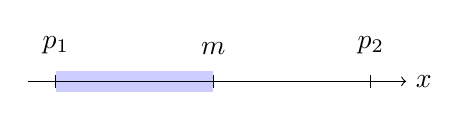
\begin{tikzpicture}[x=1cm,y=1cm]
\fill[blue!20] (0,-0.13) rectangle (2,0.13);
\draw[->] (-0.35,0) -- (4.45,0) node[right] {$x$};
\foreach \x/\lab in {0/p_1,2/m,4/p_2} {
  \draw (\x,-0.08) -- (\x,0.08);
  \node[above=4pt] at (\x,0.08) {$\lab$};
}
\end{tikzpicture}
\end{minipage}\hfill
\begin{minipage}{0.48\textwidth}
\centering
\textbf{(b) $m>p_2$}\par\smallskip
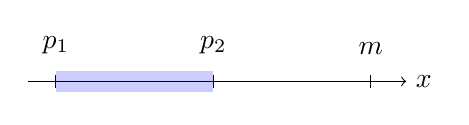
\begin{tikzpicture}[x=1cm,y=1cm]
\fill[blue!20] (0,-0.13) rectangle (2,0.13);
\draw[->] (-0.35,0) -- (4.45,0) node[right] {$x$};
\foreach \x/\lab in {0/p_1,2/p_2,4/m} {
  \draw (\x,-0.08) -- (\x,0.08);
  \node[above=4pt] at (\x,0.08) {$\lab$};
}
\end{tikzpicture}
\end{minipage}
\caption{State intervals used in the destination comparison. The shaded interval is $[p_1,h]$, where $h=\min\{m,p_2\}$.}
\label{fig:destination-comparison-intervals}
\end{figure}

Let $L(x)$ be the transformed value of always using product 1, approaching $p_1$. Let $H(x)$ be the transformed value of using product 2 to reach $h$ and then holding there. When $h=p_2$, this means approaching $p_2$ asymptotically under product 2. On $(p_1,h)$,
\begin{equation*}
\delta L=F+b_1L',\qquad \delta H=F+b_2H',
\qquad
L(p_1)=\frac{F(p_1)}{\delta},\quad
H(h)=\frac{F(h)}{\delta}.
\end{equation*}

Let $x_i(t;x)$ denote the trajectory starting from $x$ under product $i$,so that
\begin{equation*}
       \dot{x}_i(t;x)=b_i(x_i(t;x)),
       \qquad
       x_i(0;x)=x.
\end{equation*}

The preceding ODEs admit the corresponding discounted-payoff
representations
\begin{equation*}
       L(x)=\int_0^\infty e^{-\delta t}F(x_1(t;x))\,dt.
\end{equation*}

If $h<p_2$, let $\tau_h(x)$ denote the time at which the product-2 trajectory reaches $h$. Then
\begin{equation*}
       H(x)=\int_0^{\tau_h(x)}e^{-\delta t}F(x_2(t;x))\,dt+e^{-\delta\tau_h(x)}
\frac{F(h)}{\delta}.
\end{equation*}

When $h=p_2$, the product-2 trajectory approaches $p_2$ asymptotically, and the representation becomes
\begin{equation*}
       H(x)=\int_0^\infty e^{-\delta t}F(x_2(t;x))\,dt.
\end{equation*}

If $x$ is in the decreasing part of $F$ on this interval, the trajectory toward $p_1$ satisfies
\begin{equation*}
       F(x_1(t;x))>F(x),\qquad t>0,
\end{equation*}
and therefore
\begin{equation*}
       L(x)>\int_0^\infty e^{-\delta t}F(x)\,dt=\frac{F(x)}{\delta}.
\end{equation*}
Hence $\delta L(x)>F(x)$. If $x$ is in the increasing part, the analogous
comparison along the trajectory toward $h$ gives $\delta H(x)>F(x)$.
At the valley either comparison is strict. Thus
\begin{equation*}
       \delta\max\{L(x),H(x)\}>F(x),\qquad p_1<x<h.
\end{equation*}
Where $L(x)>H(x)$, the preceding inequality implies $\delta L(x)-F(x)>0$. Since $b_1(x)<0$ on $(p_1,h)$,
\begin{equation*}
       L'(x)=\frac{\delta L(x)-F(x)}{b_1(x)}<0.
\end{equation*}
Thus product 1 maximizes the Bellman expression. Similarly  where $H(x)>L(x)$,since $b_2(x)>0$ we have
\begin{equation*}
       H'(x)=\frac{\delta H(x)-F(x)}{b_2(x)}>0,
\end{equation*}
therefore, product 2 is optimal.

Now consider an interior crossing $x^*\in(p_1,h)$ such that
$L(x^*)=H(x^*)$. Using the two ODEs,
\begin{equation*}
       (H-L)'(x^*)=\bigl(\delta L(x^*)-F(x^*)\bigr)\left(\frac{1}{b_2(x^*)}-\frac{1}{b_1(x^*)}\right)>0.
\end{equation*}
Hence every interior crossing has the same orientation: $L$ wins immediately to the left and $H$ immediately to the right. There can therefore be at most one such crossing. If it occurs at $x^*$, then
\begin{equation*}
       L(x)>H(x),\qquad p_1<x<x^*,
\end{equation*}
and
\begin{equation*}
       H(x)>L(x),\qquad x^*<x<h.
\end{equation*}
Moreover, following either winning branch remains in its winning region: under product 1 the state moves toward $p_1$, while under product 2 it moves toward $h$. Endpoint ties at $p_1$ and $p_2$ are treated separately below.

% This also verifies the proposed value, without assuming a destination representation in advance. If $h=m<p_2$, an excursion above $h$ can be replaced by holding at $h$ until its return, since $F(x)\le F(h)$ for $x>h$. An excursion that never returns is likewise dominated by holding.
% If $h=p_2$, the interval $[p_1,p_2]$ is already invariant. We may therefore restrict the comparison to $[p_1,h]$. There, the continuous function $\max\{L,H\}$ satisfies the Bellman inequality along every admissible trajectory. At a corner, times spent at the corner are covered by
% $\delta\max\{L,H\}>F$; crossings of it are covered by the almost-everywhere chain rule. Integration of the discounted inequality gives an upper bound for every payoff, because the bounded terminal value vanishes. Following
% the winning branch attains this bound. Hence $W=\max\{L,H\}$ on $[p_1,h]$. A crossing may have a corner, so no smooth-fit condition is
% imposed there.

\noindent\medskip\textbf{Verification of the optimal value:}
We now verify that $\widehat W$ is the optimal value in $[p_1,h]$. Define
\begin{equation*}
    \widehat W(x)=\max\{L(x),H(x)\},
    \qquad x\in[p_1,h].
\end{equation*}
We first show that, for any initial state in $[p_1,h]$, no value is lost by restricting attention to trajectories that remain in this interval. If $h=p_2$, this follows immediately because $[p_1,p_2]$ is invariant. Suppose instead that
$h=m<p_2$. Any excursion above $h$ can be replaced by holding the state at $h$ until the original trajectory returns. Such holding is feasible because $h\in(p_1,p_2)$ and relaxed controls are allowed. Since $h=m$ is the peak
of $F$ and $F$ decreases for $x>h$,
\begin{equation*}
    F(x)\leq F(h),\qquad x>h.
\end{equation*}
Therefore, this replacement weakly increases the discounted payoff. If the trajectory never returns to $h$, holding at $h$ forever is likewise weakly better. Hence no optimal trajectory starting in $[p_1,h]$ needs to leave
this interval.

We may therefore restrict the problem to $[p_1,h]$. 
By the preceding comparison, $\widehat W$ is continuous and continuously differentiable except possibly at the unique interior crossing of $L$ and $H$. Moreover,
\begin{equation}\label{eq:candidate-holding-bound}
    \delta\widehat W(x)\geq F(x),
    \qquad x\in[p_1,h],
\end{equation}
with strict inequality for $p_1<x<h$.

At every interior point where $L\neq H$, the winning branch satisfies its Bellman equation and selects the maximizing product. Hence
\begin{equation*}
    \delta\widehat W(x)
    =
    F(x)+\max_{i=1,2}\{b_i(x)\widehat W'(x)\}.
\end{equation*}
Since the drift under a mixture is a weighted average of $b_1(x)$ and $b_2(x)$, it follows that along any admissible trajectory in $[p_1,h]$,
\begin{equation*}
    \frac{d}{dt}\widehat W(x(t))
    \leq
    \delta\widehat W(x(t))-F(x(t))
\end{equation*}
for almost every $t$. If the trajectory spends positive time at an endpoint or at the possible crossing, the same inequality follows directly from
\eqref{eq:candidate-holding-bound}.

Therefore,
\begin{equation*}
    \frac{d}{dt}
    \left[e^{-\delta t}\widehat W(x(t))\right]
    \leq
    -e^{-\delta t}F(x(t))
\end{equation*}
for almost every $t$. Integrating from $0$ to $T$ gives
\begin{equation*}
    \int_0^T e^{-\delta t}F(x(t))\,dt
    \leq
    \widehat W(x)-e^{-\delta T}\widehat W(x(T)).
\end{equation*}
Since $\widehat W$ is bounded on $[p_1,h]$, the terminal term vanishes as $T\to\infty$. Thus every admissible trajectory satisfies
\begin{equation*}
    \int_0^\infty e^{-\delta t}F(x(t))\,dt
    \leq
    \widehat W(x),
\end{equation*}
and therefore
\begin{equation*}
    W(x)\leq\widehat W(x).
\end{equation*}

Conversely, the policies defining $L$ and $H$ are admissible, so
\begin{equation*}
    W(x)\geq L(x),
    \qquad
    W(x)\geq H(x).
\end{equation*}
Hence
\begin{equation*}
    W(x)=\widehat W(x)=\max\{L(x),H(x)\},
    \qquad x\in[p_1,h].
\end{equation*}
Following the winning branch attains this value and, by the crossing orientation established above, remains in its winning region. Thus these choices define an optimal stationary policy on $[p_1,h]$.

The following figure illustrates what we have proved until now, that is,if is there any crossings in the interval $[p_1,h]$ is only in the direction $1 \rightarrow 2$. Constant policies are allowed too.

\begin{figure}[H]
\centering
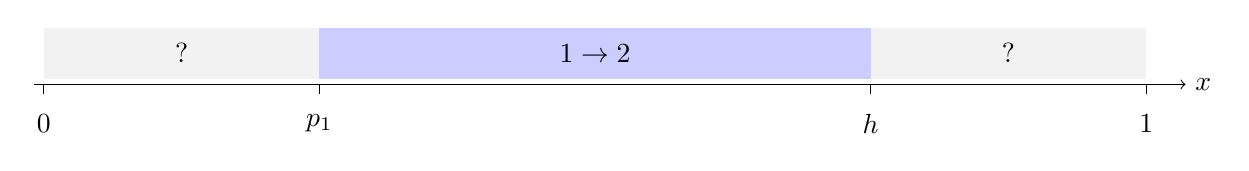
\begin{tikzpicture}[x=1cm,y=1cm]
\fill[gray!10] (0,0.07) rectangle (3.5,0.72);
\fill[blue!20] (3.5,0.07) rectangle (10.5,0.72);
\fill[gray!10] (10.5,0.07) rectangle (14,0.72);
\node at (1.75,0.395) {$?$};
\node at (7,0.395) {$1\to2$};
\node at (12.25,0.395) {$?$};
\draw[->] (-0.12,0) -- (14.5,0) node[right] {$x$};
\foreach \x/\lab in {0/0,3.5/p_1,10.5/h,14/1} {
  \draw (\x,0) -- (\x,-0.12);
  \node[below=4pt] at (\x,-0.12) {$\lab$};
}
\end{tikzpicture}
\label{fig:middle-interval-policy}
\end{figure}

\medskip\noindent\textbf{Case $m\le p_1$.}
In this case we study the regions $x\ge m$ and $x<m$ separately.

\begin{figure}[H]
\centering
\begin{minipage}{0.48\textwidth}
\centering
\textbf{(a) $x\ge m$}\par\smallskip
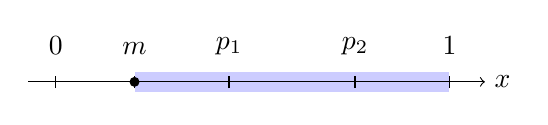
\begin{tikzpicture}[x=1cm,y=1cm]
\fill[blue!20] (1,-0.13) rectangle (5,0.13);
\draw[->] (-0.35,0) -- (5.45,0) node[right] {$x$};
\foreach \x/\lab in {0/0,1/m,2.2/p_1,3.8/p_2,5/1} {
  \draw (\x,-0.08) -- (\x,0.08);
  \node[above=4pt] at (\x,0.08) {$\lab$};
}
\fill (1,0) circle (1.8pt);
\end{tikzpicture}
\end{minipage}\hfill
\begin{minipage}{0.48\textwidth}
\centering
\textbf{(b) $x<m$}\par\smallskip
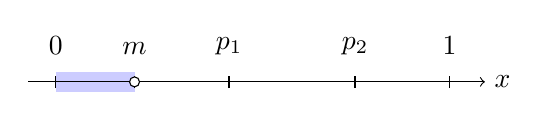
\begin{tikzpicture}[x=1cm,y=1cm]
\fill[blue!20] (0,-0.13) rectangle (1,0.13);
\draw[->] (-0.35,0) -- (5.45,0) node[right] {$x$};
\foreach \x/\lab in {0/0,1/m,2.2/p_1,3.8/p_2,5/1} {
  \draw (\x,-0.08) -- (\x,0.08);
  \node[above=4pt] at (\x,0.08) {$\lab$};
}
\draw[fill=white] (1,0) circle (1.8pt);
\end{tikzpicture}
\end{minipage}
\end{figure}

In diagram (a), for any $x\ge m$ every admissible trajectory stays in $[m,1]$. Since $F$ decreases on this interval, product 1 is optimal there by trajectory ordering.
In diagram (b), $x<m$ so Table $(*)$ permits only a $1\to2$ crossing before $a$ and only a $2\to1$ crossing between $a$ and $m$.
Within a region with only one permitted crossing orientation there can be at most one strict crossing. Thus there is at most one product-2 interval.
The same argument applies when $m=p_1$, where product 1 can hold the peak. 

This case looks like this 

\begin{figure}[H]
\centering
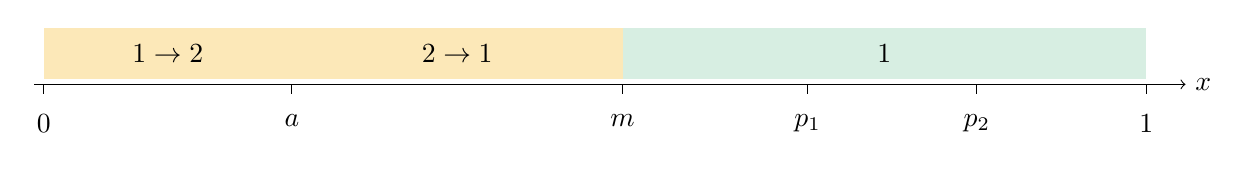
\begin{tikzpicture}[x=1cm,y=1cm]
\definecolor{policyStart}{HTML}{FCE8B8}
\definecolor{policyEnd}{HTML}{FCE8B8}
\definecolor{policyHold}{HTML}{D7EEE2}
\fill[policyStart] (0,0.07) rectangle (3.15,0.72);
\fill[policyEnd] (3.15,0.07) rectangle (7.35,0.72);
\fill[policyHold] (7.35,0.07) rectangle (14,0.72);
\node at (1.575,0.395) {$1\to2$};
\node at (5.25,0.395) {$2\to1$};
\node at (10.675,0.395) {$1$};
\draw[->] (-0.12,0) -- (14.5,0) node[right] {$x$};
\foreach \x/\lab in {0/0,3.15/a,7.35/m,9.7/p_1,11.85/p_2,14/1} {
  \draw (\x,0) -- (\x,-0.12);
  \node[below=4pt] at (\x,-0.12) {$\lab$};
}
\end{tikzpicture}
\end{figure}

\medskip\noindent\textbf{Case $p_1<m\le p_2$.}
Above $m$, product 1 is optimal. To see this, consider any admissible trajectory starting from $x>m$. Since $b_1(x)<b_2(x)$ at every state, using product 1 produces the smallest admissible trajectory and therefore reaches $m$ no later than any other trajectory that reaches $m$. Moreover, $F$ is decreasing above $m$, so before reaching $m$ the product-1 trajectory yields a weakly higher flow payoff.

If another trajectory reaches $m$ later, the product-1 trajectory can hold at $m$ until that time. During this waiting period it earns $F(m)$, which is at least the payoff of the other trajectory while it remains above $m$. Once both trajectories are at $m$, the product-1 trajectory can follow the same continuation. If the other trajectory never reaches $m$, holding at $m$ forever after arriving is likewise weakly better. Hence reaching $m$ under product 1 and then continuing optimally weakly dominates any other policy starting above $m$.

Thus product 1 is optimal for $x>m$, regardless of which continuation is optimal at $m$. On $[p_1,m]$, the preceding destination comparison gives at most one $1\to2$ crossing. Until here we have proved: 

\begin{figure}[H]
\centering
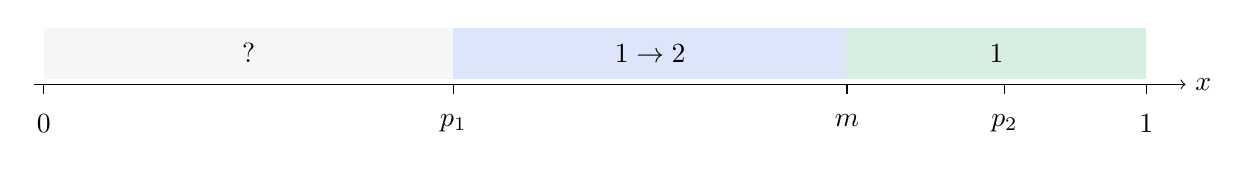
\begin{tikzpicture}[x=1cm,y=1cm]
\definecolor{policyUnknown}{HTML}{F5F6F7}
\definecolor{policyComparison}{HTML}{DDE5FA}
\definecolor{policyHold}{HTML}{D7EEE2}
\fill[policyUnknown] (0,0.07) rectangle (5.2,0.72);
\fill[policyComparison] (5.2,0.07) rectangle (10.2,0.72);
\fill[policyHold] (10.2,0.07) rectangle (14,0.72);
\node at (2.6,0.395) {$?$};
\node at (7.7,0.395) {$1\to2$};
\node at (12.1,0.395) {$1$};
\draw[->] (-0.12,0) -- (14.5,0) node[right] {$x$};
\foreach \x/\lab in {0/0,5.2/p_1,10.2/m,12.2/p_2,14/1} {
  \draw (\x,0) -- (\x,-0.12);
  \node[below=4pt] at (\x,-0.12) {$\lab$};
}
\end{tikzpicture}
\end{figure}

% There cannot be a detached product-2 interval below $p_1$. If $a\ge p_1$, then $F'<0$ below $p_1$, where table $(*)$ allows only $1\to2$ crossings. If the low branch wins at $p_1$, then $g(p_1)=0$ and $F'(p_1)<0$.
% A product-2 interval immediately to its left would have $g>0$ and use $b_2>0$, so $g'=\delta g/b_2-F'>0$ near $p_1$; this contradicts $g(p_1)=0$. Thus no left product-2 interval can occur and disappear there. If the high branch strictly wins at $p_1$, then $g(p_1)>0$ and
% continuity attaches the left product-2 interval to the high branch. Endpoint ties are detailed below.
% If instead $a<p_1$, then for every $x\in(a,p_1)$, even approaching $p_1$ under product 1 gives strictly higher subsequent $F$ than $F(x)$.
% Consequently $g(x)>0$ and $W'(x)>0$ throughout this segment. Before $a$, only a $1\to2$ crossing is possible. This again gives attachment rather
% than a second interval. If $a=p_1$, the high destination strictly improves on holding at the valley, so it wins at $p_1$ and the same argument applies.
% This proves the claim for this case, including $m=p_2$, which is held with pure product 2 if the high destination is chosen.

Now we prove that there cannot be a detached product-2 interval below $p_1$.
Suppose first that $a>p_1$. Then $F'<0$ below $p_1$, so table $(*)$
allows only $1\to2$ crossings in this region. If the low branch wins at
$p_1$, then
\begin{equation*}
    g(p_1)=0,
    \qquad
    F'(p_1)<0.
\end{equation*}
If product 2 were optimal immediately to the left of $p_1$, then
$g>0$ and the active drift would be $b_2>0$. Hence
\begin{equation*}
    g'=\frac{\delta g}{b_2}-F'>0
\end{equation*}
near $p_1$, which is incompatible with $g$ approaching
$g(p_1)=0$ from positive values. Thus product 1 is optimal immediately
to the left of $p_1$. Since no $2\to1$ crossing is possible below $p_1$,
there can be no product-2 interval there.

\begin{figure}[H]
\centering
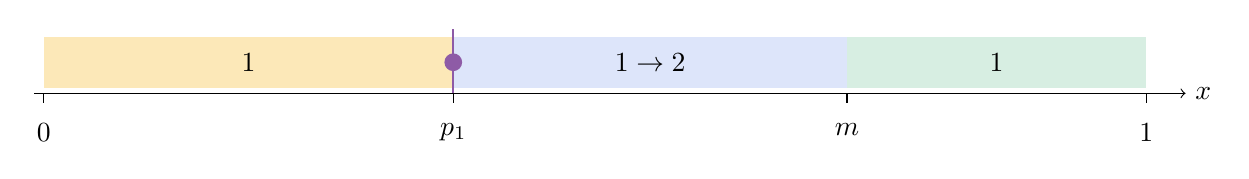
\begin{tikzpicture}[x=1cm,y=1cm]
\definecolor{policyLow}{HTML}{FCE8B8}
\definecolor{policyComparison}{HTML}{DDE5FA}
\definecolor{policyHold}{HTML}{D7EEE2}
\definecolor{policyBoundary}{HTML}{8E5BA6}
\fill[policyLow] (0,0.07) rectangle (5.2,0.72);
\fill[policyComparison] (5.2,0.07) rectangle (10.2,0.72);
\fill[policyHold] (10.2,0.07) rectangle (14,0.72);
\draw[policyBoundary,line width=0.8pt] (5.2,0) -- (5.2,0.82);
\fill[policyBoundary] (5.2,0.395) circle (3.2pt);
\node at (2.6,0.395) {$1$};
\node at (7.7,0.395) {$1\to2$};
\node at (12.1,0.395) {$1$};
\draw[->] (-0.12,0) -- (14.5,0) node[right] {$x$};
\foreach \x/\lab in {0/0,5.2/p_1,10.2/m,14/1} {
  \draw (\x,0) -- (\x,-0.12);
  \node[below=4pt] at (\x,-0.12) {$\lab$};
}
\end{tikzpicture}
\end{figure}

If instead the high branch strictly wins at $p_1$, then $g(p_1)>0$.
By continuity, product 2 is also optimal immediately to the left of
$p_1$. Since only a $1\to2$ crossing is possible below $p_1$, any
product-2 region on the left must attach to the product-2 region above
$p_1$, rather than form a second interval. Endpoint ties are treated
separately below.

\begin{figure}[H]
\centering
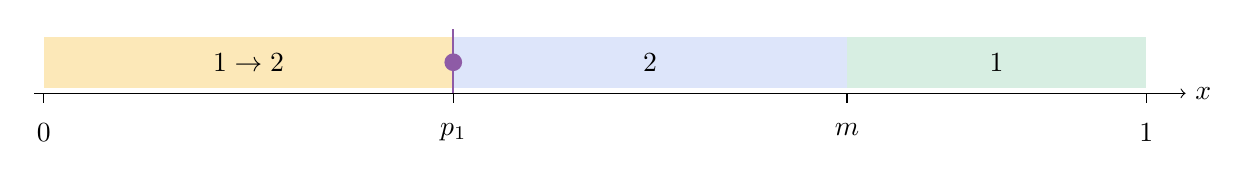
\begin{tikzpicture}[x=1cm,y=1cm]
\definecolor{policyLow}{HTML}{FCE8B8}
\definecolor{policyComparison}{HTML}{DDE5FA}
\definecolor{policyHold}{HTML}{D7EEE2}
\definecolor{policyBoundary}{HTML}{8E5BA6}
\fill[policyLow] (0,0.07) rectangle (5.2,0.72);
\fill[policyComparison] (5.2,0.07) rectangle (10.2,0.72);
\fill[policyHold] (10.2,0.07) rectangle (14,0.72);
\draw[policyBoundary,line width=0.8pt] (5.2,0) -- (5.2,0.82);
\fill[policyBoundary] (5.2,0.395) circle (3.2pt);
\node at (2.6,0.395) {$1\to2$};
\node at (7.7,0.395) {$2$};
\node at (12.1,0.395) {$1$};
\draw[->] (-0.12,0) -- (14.5,0) node[right] {$x$};
\foreach \x/\lab in {0/0,5.2/p_1,10.2/m,14/1} {
  \draw (\x,0) -- (\x,-0.12);
  \node[below=4pt] at (\x,-0.12) {$\lab$};
}
\end{tikzpicture}
\end{figure}

Now suppose that $a<p_1$. For every $x\in(a,p_1)$, using product 1 to
move toward $p_1$ yields strictly higher subsequent values of $F$ than
$F(x)$. Therefore,
\begin{equation*}
    W(x)>\frac{F(x)}{\delta},
\end{equation*}
so $g(x)>0$. Since both drifts are positive below $p_1$, this implies
$W'(x)>0$, and product 2 is optimal throughout $(a,p_1)$. Before $a$,
table $(*)$ again allows only a $1\to2$ crossing, so any product-2
region there must attach to $(a,p_1)$.

\begin{figure}[H]
\centering
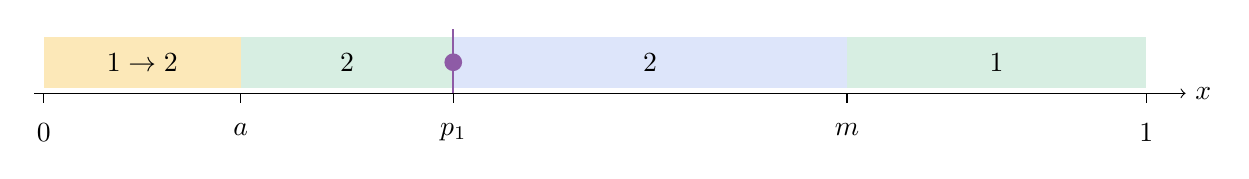
\begin{tikzpicture}[x=1cm,y=1cm]
\definecolor{policyLow}{HTML}{FCE8B8}
\definecolor{policyComparison}{HTML}{DDE5FA}
\definecolor{policyHold}{HTML}{D7EEE2}
\definecolor{policyBoundary}{HTML}{8E5BA6}
\fill[policyLow] (0,0.07) rectangle (2.5,0.72);
\fill[policyHold] (2.5,0.07) rectangle (5.2,0.72);
\fill[policyComparison] (5.2,0.07) rectangle (10.2,0.72);
\fill[policyHold] (10.2,0.07) rectangle (14,0.72);
\draw[policyBoundary,line width=0.8pt] (5.2,0) -- (5.2,0.82);
\fill[policyBoundary] (5.2,0.395) circle (3.2pt);
\node at (1.25,0.395) {$1\to2$};
\node at (3.85,0.395) {$2$};
\node at (7.7,0.395) {$2$};
\node at (12.1,0.395) {$1$};
\draw[->] (-0.12,0) -- (14.5,0) node[right] {$x$};
\foreach \x/\lab in {0/0,2.5/a,5.2/p_1,10.2/m,14/1} {
  \draw (\x,0) -- (\x,-0.12);
  \node[below=4pt] at (\x,-0.12) {$\lab$};
}
\end{tikzpicture}
\end{figure}

Finally, if $a=p_1$, then $p_1$ is the valley of $F$. Moving toward the
higher destination strictly improves on holding at $p_1$, so the high
branch wins there and the same attachment argument applies. Hence in
all cases product 2 can form at most one interval below and across
$p_1$. 

The conclusion of this part can be illustrated it as follows: 

\begin{figure}[H]
\centering
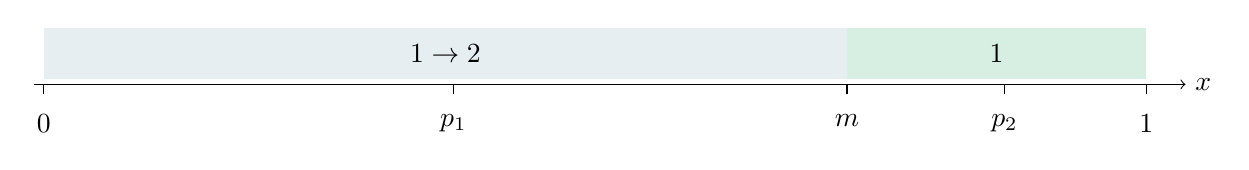
\begin{tikzpicture}[x=1cm,y=1cm]
\definecolor{policyJoined}{HTML}{E7EEF2}
\definecolor{policyHold}{HTML}{D7EEE2}
\fill[policyJoined] (0,0.07) rectangle (10.2,0.72);
\fill[policyHold] (10.2,0.07) rectangle (14,0.72);
\node at (5.1,0.395) {$1\to2$};
\node at (12.1,0.395) {$1$};
\draw[->] (-0.12,0) -- (14.5,0) node[right] {$x$};
\foreach \x/\lab in {0/0,5.2/p_1,10.2/m,12.2/p_2,14/1} {
  \draw (\x,0) -- (\x,-0.12);
  \node[below=4pt] at (\x,-0.12) {$\lab$};
}
\end{tikzpicture}
\end{figure}

\medskip\noindent\textit{Case $m>p_2$.}
% On $[p_1,p_2]$ the destination comparison applies with $h=p_2$.
% The preceding argument below $p_1$ is unchanged.
% If $a\ge p_2$, every trajectory starting at $x\le a$ stays below $a$,
% where $F$ decreases; product 1 is optimal there. Above $a$, table $(*)$
% allows only $1\to2$ crossings up to $m$ and only $2\to1$ crossings
% afterward. There is at most one product-2 interval, entirely on the right.

% If $a<p_2$, then $F'>0$ on $(p_2,m)$, so table $(*)$ allows only
% $1\to2$ crossings there. If the high destination wins at $p_2$, then $g(p_2)=0$.
% An interval of product 1 immediately on its right would have $g>0$
% and satisfy $g'=\delta g/b_1-F'<0$ near $p_2$, which cannot emerge
% from zero. Thus its product-2 interval continues to the right and cannot
% split before $m$. If the low destination wins at $p_2$, no product-2 interval
% can have ended earlier inside $[p_1,p_2]$, since all middle crossings
% have orientation $1\to2$. Any later product-2 interval is then the only
% one. Beyond $m$, table $(*)$ allows it to end at most once.

On $[p_1,p_2]$, the destination comparison applies with $h=p_2$, and the
preceding argument below $p_1$ is unchanged.

Suppose first that $a\geq p_2$. Any trajectory starting at $x\leq a$ remains below $a$, where $F$ is decreasing. Since product 1 generates the
smallest admissible trajectory, it is optimal throughout this region. For $x>a$, table $(*)$ allows only $1\to2$ crossings on $(a,m)$ and only
$2\to1$ crossings on $(m,1)$. Hence product 2 can be optimal on at most one interval.


\begin{figure}[H]
\centering
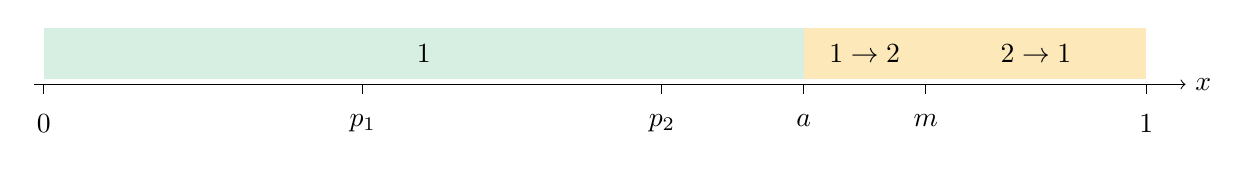
\begin{tikzpicture}[x=1cm,y=1cm]
\definecolor{policyHold}{HTML}{D7EEE2}
\definecolor{policyLow}{HTML}{FCE8B8}
\fill[policyHold] (0,0.07) rectangle (9.65,0.72);
\fill[policyLow] (9.65,0.07) rectangle (11.2,0.72);
\fill[policyLow] (11.2,0.07) rectangle (14,0.72);
\node at (4.825,0.395) {$1$};
\node at (10.425,0.395) {$1\to2$};
\node at (12.6,0.395) {$2\to1$};
\draw[->] (-0.12,0) -- (14.5,0) node[right] {$x$};
\foreach \x/\lab in {0/0,4.05/p_1,7.85/p_2,9.65/a,11.2/m,14/1} {
  \draw (\x,0) -- (\x,-0.12);
  \node[below=4pt] at (\x,-0.12) {$\lab$};
}
\end{tikzpicture}
\end{figure}


Now suppose that $a<p_2$. Then $F'>0$ on $(p_2,m)$, so table $(*)$ allows
only $1\to2$ crossings there. If the high destination strictly wins at
$p_2$, then
\begin{equation*}
    W(p_2)=H(p_2)=\frac{F(p_2)}{\delta},
\end{equation*}
and hence $g(p_2)=0$. Product 1 immediately to the right would require
$g>0$. On that branch, however,
\begin{equation*}
    g'=\frac{\delta g}{b_1}-F'<0,
\end{equation*}
since $b_1<0$ and $F'>0$. Thus a positive $g$ cannot emerge from $g(p_2)=0$, so product 2 remains optimal immediately to the right of $p_2$. Since no $2\to1$ crossing is possible before $m$, this product-2
region cannot split before reaching $m$.


\begin{figure}[H]
\centering
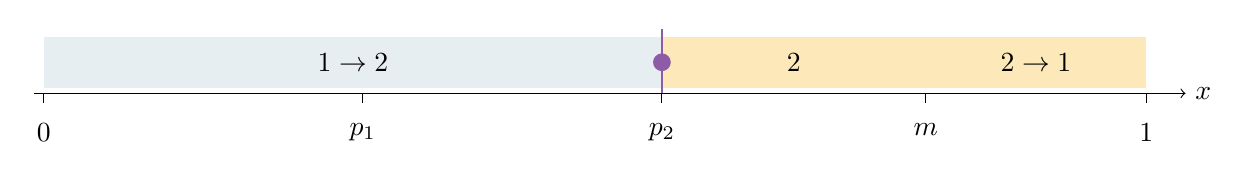
\begin{tikzpicture}[x=1cm,y=1cm]
\definecolor{policyJoined}{HTML}{E7EEF2}
\definecolor{policyLow}{HTML}{FCE8B8}
\definecolor{policyBoundary}{HTML}{8E5BA6}
\fill[policyJoined] (0,0.07) rectangle (7.85,0.72);
\fill[policyLow] (7.85,0.07) rectangle (11.2,0.72);
\fill[policyLow] (11.2,0.07) rectangle (14,0.72);
\draw[policyBoundary,line width=0.8pt] (7.85,0) -- (7.85,0.82);
\fill[policyBoundary] (7.85,0.395) circle (3.2pt);
\node at (3.925,0.395) {$1\to2$};
\node at (9.525,0.395) {$2$};
\node at (12.6,0.395) {$2\to1$};
\draw[->] (-0.12,0) -- (14.5,0) node[right] {$x$};
\foreach \x/\lab in {0/0,4.05/p_1,7.85/p_2,11.2/m,14/1} {
  \draw (\x,0) -- (\x,-0.12);
  \node[below=4pt] at (\x,-0.12) {$\lab$};
}
\end{tikzpicture}
\end{figure}

If instead the low destination strictly wins at $p_2$, then it wins throughout $[p_1,p_2]$, since any interior crossing has orientation $L\to H$. Starting from product 1 at $p_2$, table $(*)$ allows at most one $1\to2$ crossing before $m$. Beyond $m$, only a $2\to1$ crossing is possible. Hence again product 2 is optimal on at most one interval. Endpoint ties at $p_2$ are treated separately below.

\begin{figure}[H]
\centering
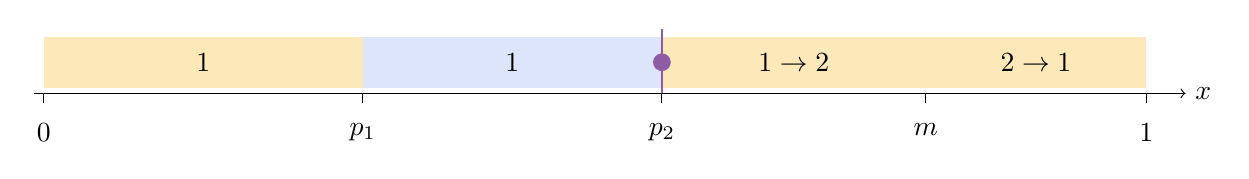
\begin{tikzpicture}[x=1cm,y=1cm]
\definecolor{policyLow}{HTML}{FCE8B8}
\definecolor{policyComparison}{HTML}{DDE5FA}
\definecolor{policyBoundary}{HTML}{8E5BA6}
\fill[policyLow] (0,0.07) rectangle (4.05,0.72);
\fill[policyComparison] (4.05,0.07) rectangle (7.85,0.72);
\fill[policyLow] (7.85,0.07) rectangle (11.2,0.72);
\fill[policyLow] (11.2,0.07) rectangle (14,0.72);
\draw[policyBoundary,line width=0.8pt] (7.85,0) -- (7.85,0.82);
\fill[policyBoundary] (7.85,0.395) circle (3.2pt);
\node at (2.025,0.395) {$1$};
\node at (5.95,0.395) {$1$};
\node at (9.525,0.395) {$1\to2$};
\node at (12.6,0.395) {$2\to1$};
\draw[->] (-0.12,0) -- (14.5,0) node[right] {$x$};
\foreach \x/\lab in {0/0,4.05/p_1,7.85/p_2,11.2/m,14/1} {
  \draw (\x,0) -- (\x,-0.12);
  \node[below=4pt] at (\x,-0.12) {$\lab$};
}
\end{tikzpicture}
\end{figure}


\medskip\noindent\textit{Endpoint ties and threshold choices.}
The preceding strict comparisons also cover roots of $F'$ at $p_1$ or
$p_2$: a valley at $p_1$ strictly favors the high destination; a valley at
$p_2$ strictly favors moving downward; peaks at either endpoint were
included in the first two cases.
For completeness, suppose $L(p_1)=H(p_1)$ with $h>p_1$.
Under the stated strict shape this requires $F'(p_1)<0$.
Here $H'(p_1)=0$ and $L'(p_1)<0$, so $H$ wins immediately to the right.
On the left, a positive $g$ would select the nonvanishing drift $b_2$ and
satisfy $g'=\delta g/b_2-F'>0$ near $p_1$, so could not reach
$g(p_1)=0$ from positive values. The left side therefore uses product 1;
the tie creates one $1\to2$ switch, not another interval.
Likewise, a tie at $p_2$ when $m>p_2$ requires $F'(p_2)>0$.
Here $L'(p_2)=0<H'(p_2)$, so $L$ wins immediately to the left.
Immediately on the right, a positive $g$, which would select $b_1<0$,
would satisfy $g'=\delta g/b_1-F'<0$ and cannot emerge from
$g(p_2)=0$. Hence that side selects product 2. Again the switch is
$1\to2$ and introduces no detached interval.

At an interior tie between destinations, select either destination.
At an attractive peak $m\in(p_1,p_2)$, holding uses the fraction
$(m-p_1)/(p_2-p_1)$ of product 2. With these threshold choices the policy
attains the value and has at most one interval of product-2 use, as claimed.
\end{proof}

\begin{proof}[Proof of Proposition~\ref{prop:fluid-band}]
The transformation \eqref{eq:transform} preserves the ranking of every
admissible policy from a given initial state. Lemma~\ref{lem:beta-marginal-demand}
and Lemma~\ref{lem:F-shape} establish the required payoff shape for the exact
Beta demand. The preceding control lemma gives an optimal policy with at
most one product-2 interval. Translating back to $V$ leaves that policy
unchanged and proves the proposition.
\end{proof}

\section*{4. When at least one threshold must exist}
An upper bound on the number of thresholds does not guarantee that any
threshold exists. The following fixed-policy tests distinguish the two
constant-policy cases. Write $U^i_\rho$ for the fluid value obtained by
always using product $i$:
\begin{equation*}
U^i_\rho(x)=(R-c_i)\int_0^\infty e^{-\delta t}D(x_i(t;x))\,dt.
\end{equation*}
These functions are continuously differentiable. Indeed, fixed-policy
trajectories converge uniformly exponentially to $p_i$, and their initial
state derivatives are positive and eventually decay exponentially. One
can therefore differentiate this integral under the integral sign.

\begin{corollary}[Existence of a nonconstant threshold policy]
Under the assumptions of Proposition~\ref{prop:fluid-band}, a nonconstant
optimal policy is necessary exactly when
\begin{align*}
\max_{x\in[0,1]}\{-\Delta c+\lambda\Delta p(U^1_\rho)'(x)\}&>0,\\
\min_{x\in[0,1]}\{-\Delta c+\lambda\Delta p(U^2_\rho)'(x)\}&<0.
\end{align*}
When both inequalities hold, there is an optimal policy with either one
or two interior thresholds, with one of the three patterns in the proposition.
\end{corollary}
\begin{proof}
The fixed-policy equations are
\begin{equation*}
\delta U^i_\rho=D(x)\{R-c_i+\lambda(p_i-x)(U^i_\rho)'\}.
\end{equation*}
If the first maximum is nonpositive, the equation for $U^1_\rho$ also
satisfies the optimal Hamiltonian inequality for product 2. Integrating
that inequality along any admissible trajectory proves that its payoff
is at most $U^1_\rho$. Thus always using product 1 is optimal everywhere.
Conversely, at a state where the expression is positive, use product 2
for a short time $h$ and then product 1 forever. Its value is
\begin{equation*}
U^1_\rho(x)+hD(x)\{-\Delta c+\lambda\Delta p(U^1_\rho)'(x)\}+o(h),
\end{equation*}
which is strictly larger for small $h>0$. Thus the first strict inequality
is equivalent to excluding the globally optimal constant policy 1.
The same argument, reversing the roles of the products, shows that the
second strict inequality excludes the globally optimal constant policy 2.
The proposition then leaves only the three nonconstant patterns.
\end{proof}

\section*{5. Interpreting the thresholds}
The arrows above describe actions as the state $x$ increases, not a
chronological sequence of purchases. At an attractive upper threshold
$x_H\in(p_1,p_2)$, holding the state requires the product-2 fraction
\begin{equation*}
\frac{x_H-p_1}{p_2-p_1}.
\end{equation*}
With only pure actions in continuous time, rapid alternation approximates
this relaxed value; a pure stationary action cannot hold at such a point.
Thus exact attainment must be stated with this convention.

A sustainable interior upper threshold is a local maximum of $F$ and
therefore satisfies
\begin{equation*}
\left[R-c_1+\frac{\Delta c}{\Delta p}(p_1-x_H)\right]D'(x_H)
=\frac{\Delta c}{\Delta p}\left[D(x_H)+\frac\delta\lambda\right].
\end{equation*}
A lower threshold need not satisfy this equation. When it separates a
trajectory toward $p_1$ from one toward a higher destination, the two
continuation values coincide but their derivatives can differ. In that
case $V$ has a corner, and imposing
$V'(x)=\Delta c/(\lambda\Delta p)$ at the threshold would be incorrect.
Thresholds outside $[p_1,p_2]$ are passage points rather than sustainable
destinations, and are determined by continuation-value matching.

The result proves the complete bound on policy patterns for this fluid
model. It does not give elementary closed-form threshold locations or
parameter boundaries, and it does not prove the same bound for the
original stochastic model.
\end{document}
